\tikzset{
  % ----- the static part of the style
  neuron/.style={
    circle,draw=black, thick, fill = white, minimum size=20,
  },
  % ----- the prescribed part pf the style
  stim/.style = {fill=blue!35,opacity=1},
  inhibit/.style = {fill=red!35,opacity=1},
  output/.style = {fill=green!35,opacity=1},
  inactive/.style = {opacity=0.5},
  hidden/.style = {draw=none},
  active/.style = {opacity=1},
  3_S1_1/.style = {stim},
%   3_S2_1/.style = {inhibit},
%   3_S3_1/.style = {inhibit},
  3_S1_2/.style = {inhibit},
  3_S2_2/.style = {stim},
  3_S3_2/.style = {stim},
%   3_S1_4/.style = {inhibit},
  3_S2_4/.style = {stim},
%   3_S3_4/.style = {inhibit},
  3_S1_5/.style = {inhibit},
  3_S2_5/.style = {stim},
  3_S3_5/.style = {inhibit}
}

\begin{figure}[!h]
    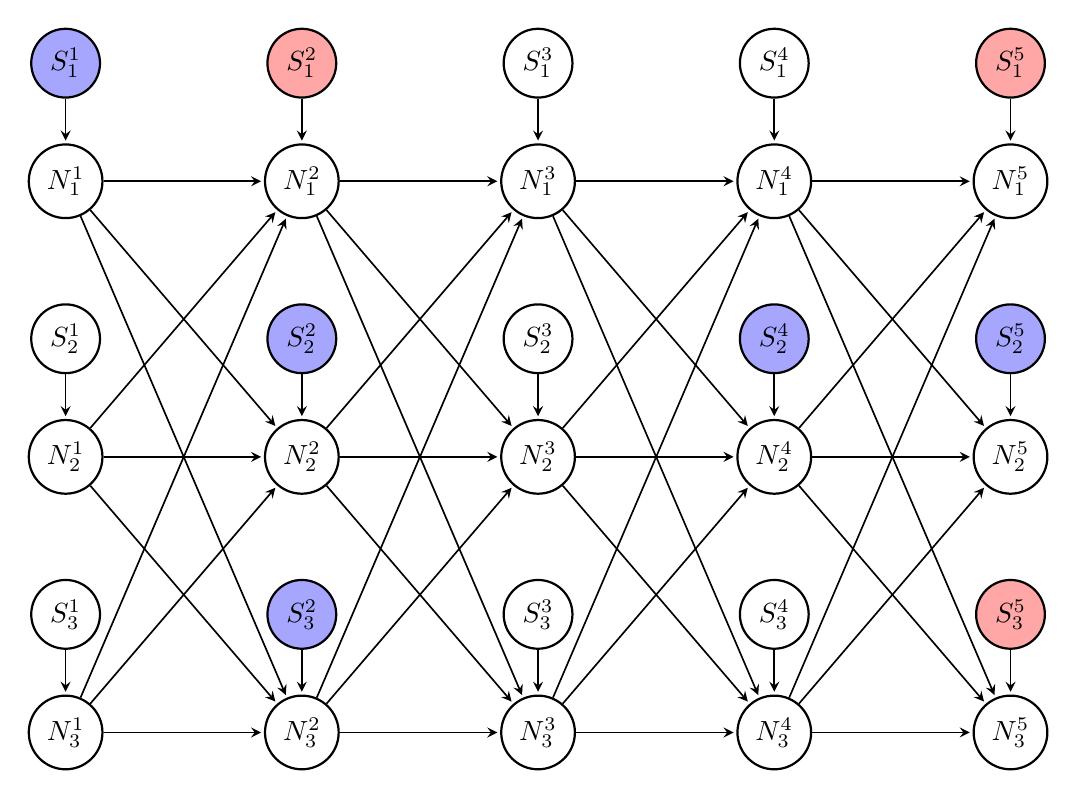
\begin{tikzpicture}[
                > = stealth, % arrow head style
                shorten > = 1pt, % don't touch arrow head to node
                auto,
                node distance = 3cm, % distance between nodes
                semithick % line style
            ]
        \tikzstyle{neuron}=[
                circle,
                draw = black,
                thick,
                fill = white,
                minimum size = 6mm
            ]
        \tikzstyle{annot} = [text width=4em, text centered]

        % t=1
        \foreach \t in {1,...,5}{
            \foreach \n in {1,...,3}{
              % stimulation
              \node[neuron,3_S\n_\t/.try] (S\n-\t) at (\t*3,-\n*3.5) {$S_\n^\t$};
              % neurons
              \node[neuron,3_N\n_\t/.try] (N\n-\t) at (\t*3,-\n*3.5-1.5) {$N_\n^\t$};
              \path[->] (S\n-\t) edge (N\n-\t);
            }
        }

        % Connect every node in t to t+1
        \foreach \source in {1,...,3}{
            \foreach \dest in {1,...,3}{
            	\foreach \t [evaluate = \t as \tt using int(\t+1)] in {1,...,4}{
                    \path[->] (N\source-\t) edge (N\dest-\tt);
                }
            }
        }
    \end{tikzpicture}
    \caption{Implementation of LTP \& LTD using excitation (blue) and inhibition (red). Starting at time 1, the synapses $(N_1,N_2)$ and $(N_1,N_3)$ undergo LTP while $(N_1,N_1)$ undergoes LTD. At time 4, the synapse $(N_2,N_2)$ undergoes LTP while $(N_2,N_1)$ and $(N_2,N_3)$ undergo LTD.}
\end{figure}
